
\section{Genetic drift}

\begin{frame}{Intended Learning Outcomes}

	\underline{Genetic drift}

	\bigskip

	In this lecture you will learn
	\begin{itemize}
		\item to describe the Wright-Fisher model of genetic drift
		\item to calculate expected allele frequencies
		\item to quantify the effect of population size on drift
	\end{itemize}

\end{frame}

\begin{frame}{Allele frequencies through time}

	Population genetics often focuses on describing the changes of allele frequencies through time.

	\bigskip
	The two most important factors that cause allele frequencies to change are
	\begin{itemize}
		\item natural selection
		\item mutations
		\item \textbf{genetic drift}
	\end{itemize}

\end{frame}


\begin{frame}{Genetic drift}

	\small
	\begin{block}{}
		The \textbf{random} change of allele frequencies in populations of \textbf{finite} size.
	\end{block}

	\pause

	\begin{columns}

                \column{0.4\textwidth}

                \begin{figure}
                        \includegraphics[width=0.8\textwidth]{Pics/population}
                \end{figure}

                \column{0.6\textwidth}
                \small

                \begin{itemize}
                        \item some individuals leave many offspring, others fewer, other none
			\item heterozygous individuals will randomly transmit allele $A$ or $a$
			\item it is very likely that allele frequencies will change from one generation to another
			\item over many generations, this process can produce large changes in allele frequencies
                \end{itemize}

        \end{columns}

\end{frame}


\begin{frame}{Wright-Fisher model}

	\begin{columns}

                \column{0.5\textwidth}

                \begin{figure}
                        \includegraphics[width=0.5\textwidth]{Pics/wright} \\
			\caption{Sewall Wright}
                \end{figure}

                \column{0.5\textwidth}

 		\begin{figure}
                        \includegraphics[width=0.5\textwidth]{Pics/fisher} \\
                        \caption{R.A. Fisher}
                \end{figure}

        \end{columns}

\end{frame}


\begin{frame}{Wright-Fisher model}

	Assumptions:
	\begin{itemize}
		\item haploid population
		\item asexual (no mating)
		\item discrete generations
	\end{itemize}

	\begin{block}{}
	In a population of size $2N$, gene copies are transmitted from generation $t$ to $t+1$ by
	random sampling with replacement (independently and with equal probability) of the gene
	copies in generation $t$.
	\end{block}

\end{frame}


\begin{frame}{Wright-Fisher model}

	\begin{figure}
        	\includegraphics[width=0.5\textwidth]{Pics/wf} \\
                \caption{Two generations of a Wright-Fisher population.}
        \end{figure}

\end{frame}


\begin{frame}{Wright-Fisher model}

	\begin{itemize}
		\item The distribution of offspring in generation $t+1$ is given by a \textbf{binomial} distribution
		\item Under the Wright-Fisher model, we can easily characterise the change in allele frequency mathematically.
	\end{itemize}

	\small
	e.g. what is the probability that any gene copy in generation $t+1$ is $A$?

	\bigskip
	\tiny{jupyter-notebook: drift}

\end{frame}


\begin{frame}{Expected allele frequency}

	What is the probability that any gene copy in generation $t+1$ is $A$?

	\begin{equation}
		E[f_a(t+1)] = 2Nf_A(t) / 2N = f_A(t)
	\end{equation}

	\begin{block}{}
		The \textbf{expected} allele frequency in generation $t+1$ is equal to the allele frequency in generation $t$.
	\end{block}


\end{frame}


\begin{frame}{Drift in the Wright-Fisher model}

	What happens when we repeat the Wright-Fisher sampling scheme over \textbf{many} generations?

	\bigskip
	\tiny{jupyter-notebook: drift}

\end{frame}


\begin{frame}{Drift in the Wright-Fisher model}

	\begin{itemize}
		\item at each generation, allele frequency might change a bit
		\item small changes add up and, after many generations, allele frequency may have changed significantly
	\end{itemize}

	\begin{block}{}
		Many small changes may result in large evolutionary changes over sufficiently long periods of time.
	\end{block}

\end{frame}


\begin{frame}{Drift in the Wright-Fisher model}

	\begin{itemize}
		\item allele frequency may increase or decrease with equal probabilities
		\item in some cases, allele has become fixed $f_A(t)=0$ or lost $f_A(t)=1$
	\end{itemize}

	\begin{block}{}
		When an allele first has become fixed or lost, its frequency cannot change anymore 
		(e.g. if $f_A(t)=0$ then $f_A(t+1)=0$)
	\end{block}

	Is it always true? \pause Yes if we assume no recurrent mutation: \\
	in the absence of recurrent mutation, it can be shown mathematically that an allele must eventually become fixed or lost.

\end{frame}


\begin{frame}{Effect of population size}

	How \textbf{fast} can genetic drift change allele frequencies? \\
	It depends on the population size, $N$.

	\bigskip
	\tiny{jupyter-notebook: drift}
	\bigskip

\end{frame}

\begin{frame}{Effect of population size}

	Large changes in allele frequency are unlikely in large populations, but happen more easily by chance
	in small populations.

	\begin{block}{}
		Genetic drift works much faster in small populations than in large populations.
	\end{block}

	\bigskip

	The effect of population size on genetic drift has important implications for our understanding
	of natural populations.

\end{frame}

\begin{frame}{Bottleneck in population size}

	\small
	\begin{block}{}
		Short period of time when the population size is very small and many alleles become either fixed or loast in the population. As a consequence, much of the population genetic variation is lost.
	\end{block}

	\begin{figure}
                \includegraphics[width=0.65\textwidth]{Pics/bottleneck}
        \end{figure}

\end{frame}


\begin{frame}{Bottleneck in population size}

	\bigskip
        \begin{figure}
                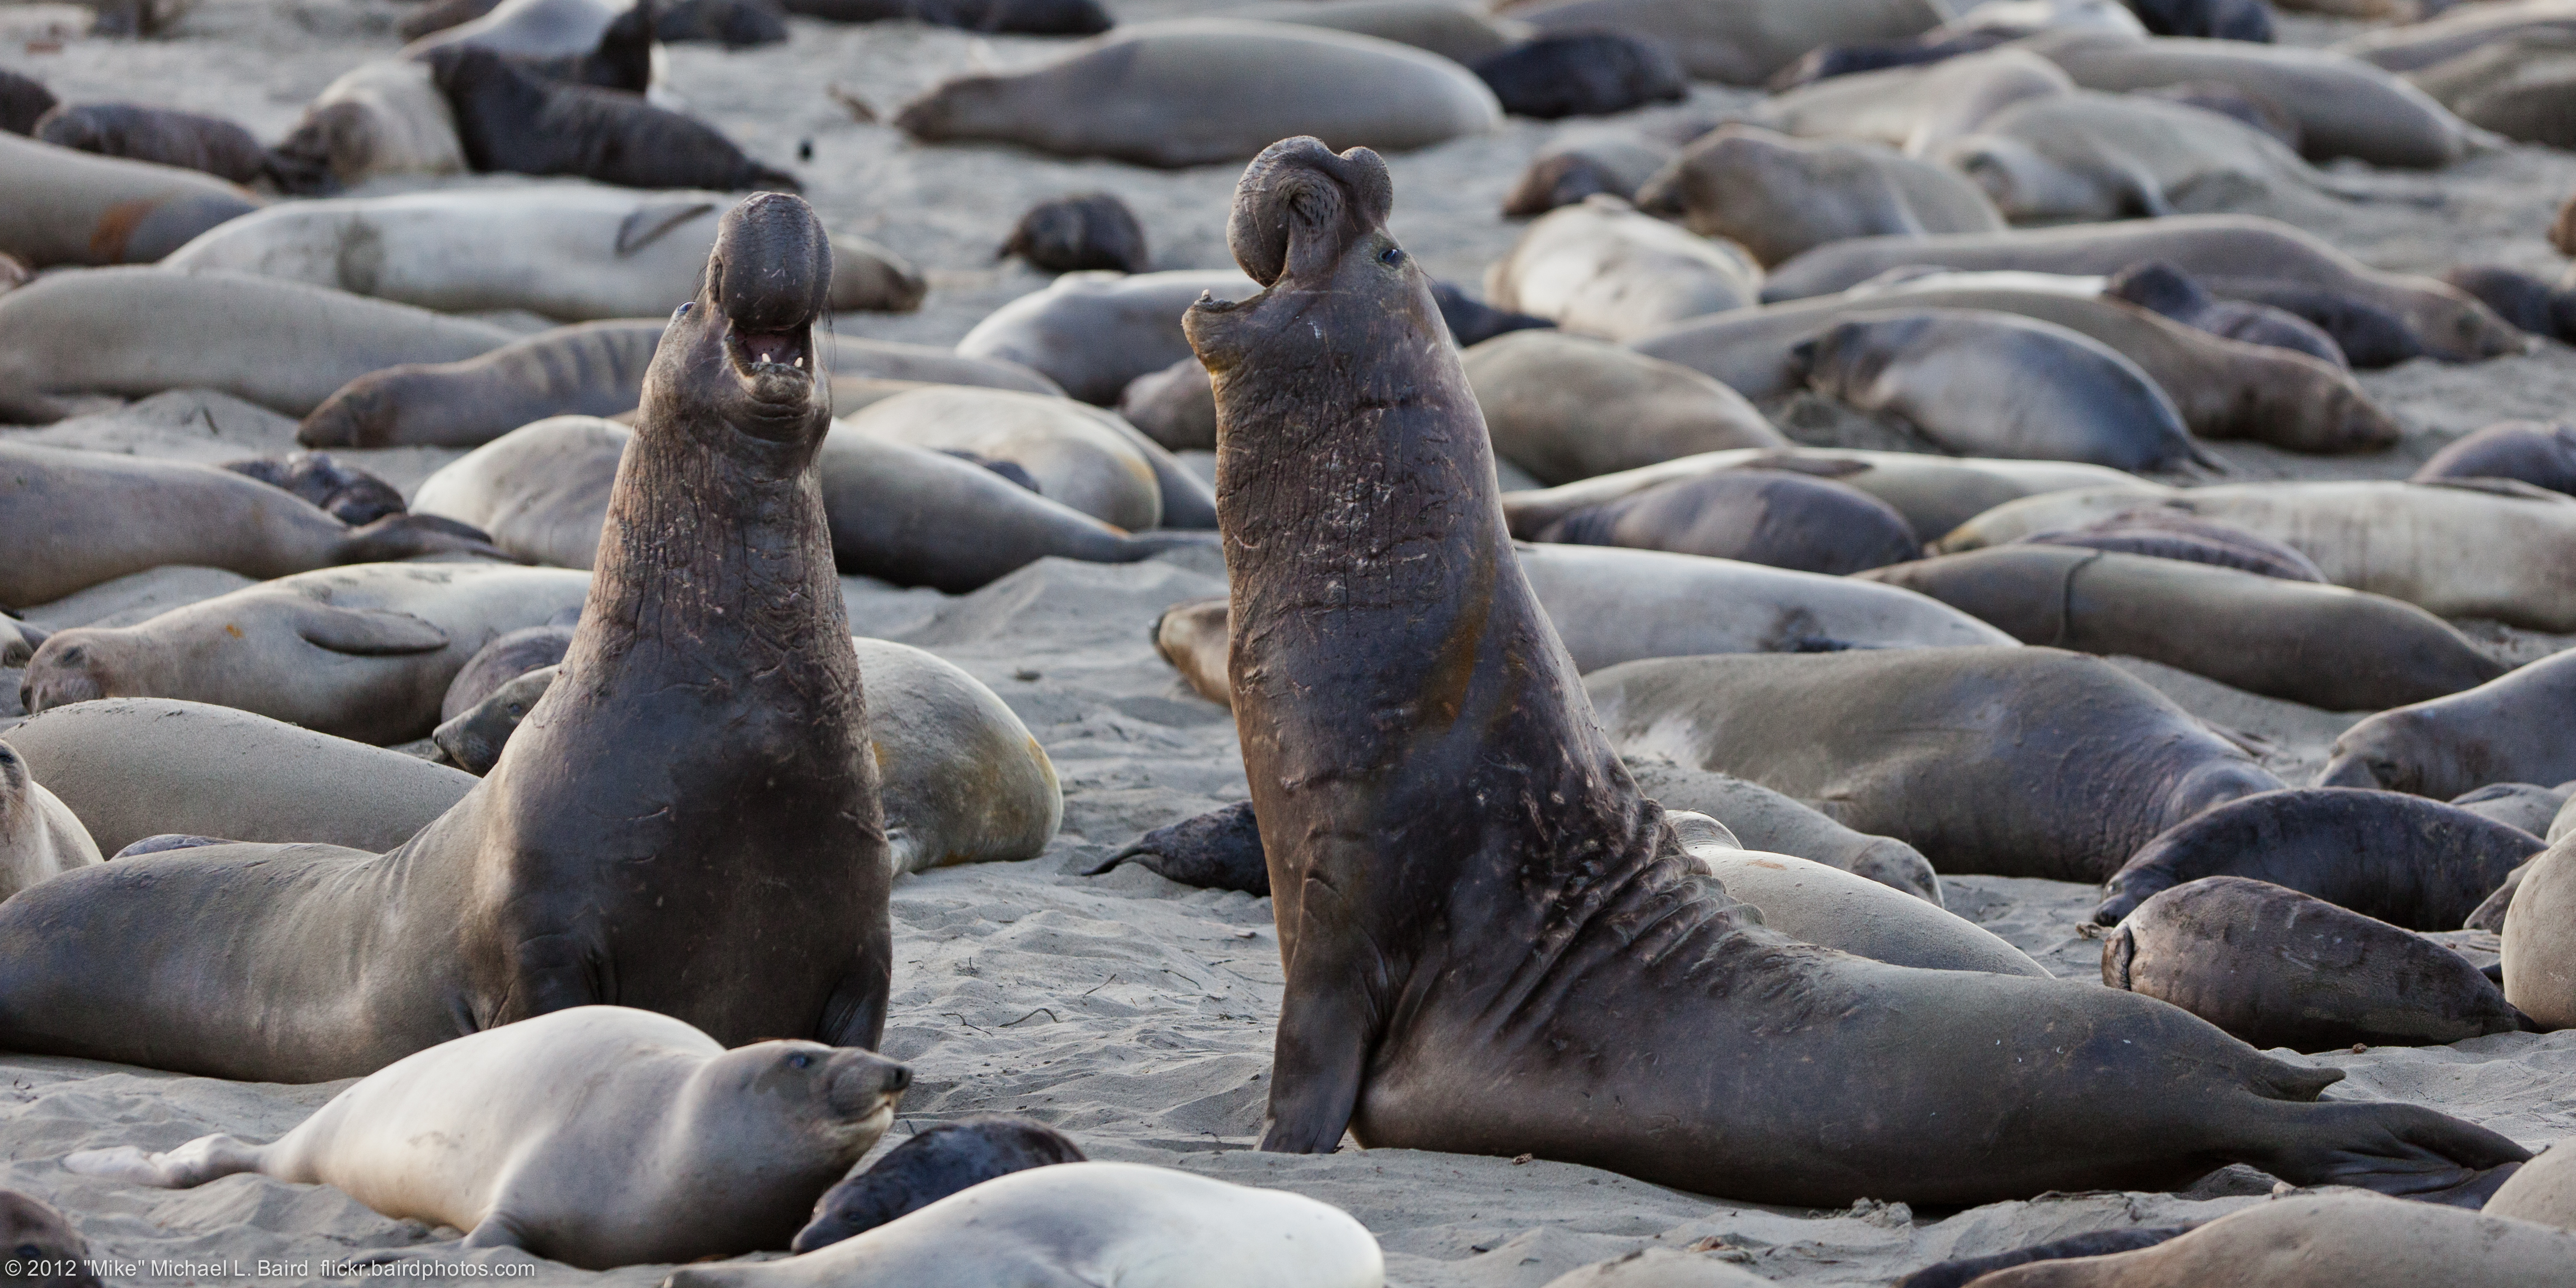
\includegraphics[width=0.55\textwidth]{Pics/elephant_seals} \\
		\caption{Northern elephant seal (\textit{Mirounga angustirostris})}
        \end{figure}

	\small
	Sea elephants were hunted nearly to extintion to a populazione of just 2-20 individuals. Today the population rebounded to 175,000 individuals.

	From historical (before hunting) and modern samples, their genetic diversity* was reduced from 0.90 to 0.41.

	\vskip 0.5cm
	\tiny * (more in this later)

\end{frame}


\begin{frame}{Founder effect}

	\bigskip
	\begin{block}{}
		Reduction in variability caused by a bottleneck in the population size during the founding of a new population.
	\end{block}

	\begin{figure}
                \includegraphics[width=0.65\textwidth]{Pics/founder}
        \end{figure}

\end{frame}


\begin{frame}{Founder effect}

        \begin{figure}
                \includegraphics[width=0.65\textwidth]{Pics/founder}
        \end{figure}

	Genetic divergence after speciation may be helped along by the \textbf{strong} effects of genetic drift in the
	founders of a population.

\end{frame}


\begin{frame}{Intended Learning Outcomes}

	\underline{Genetic drift}

        \bigskip

        In this lecture you have learnt
        \begin{itemize}
                \item to describe the Wright-Fisher model of genetic drift
                \item to calculate expected allele frequencies
                \item to quantify the effect of population size on drift
        \end{itemize}

\end{frame}




